\documentclass[12pt]{article}

\usepackage[portuguese]{babel}
\usepackage{graphicx}

\graphicspath{ {figures} }

\author{João Vitor Maia Neves Cordeiro}
\title{Segundo trabalho prática: Wiresharke e SNMP}
\date{\today}

\begin{document}

\maketitle

\begin{abstract}
O presente trabalho visa demonstrar a utilização de ferramentas de gerenciamento de rede como o PRTG e o Wireshark, a fim de dar ao leitor o material necessário para compreender o uso desses softwares e replicar os experimentos realizados. Com o uso dos programas foi realizado um monitoramento durante 3 dias com interrupções, sempre em um intervalo mínimo de duas horas a cada dia. Durante o monitoramento foram compreendidos conceitos importantes sobre os protocolos utilizados como ARP, SNMP e UDP; Além disso, essa atividade também proporcionou um entendimento de como gerenciar uma rede doméstica, verificando a eficiência da rede.
\end{abstract}

\section{Introdução}

O monitoramento de rede é de suma importância quando discutimos sobre Quality of Service (QoS) e segurança preventiva contra ataques cibernéticos. Nesse relatório será demonstrado o trabalho prático realizado utilizando as ferramentas PRTG e Wireshark, um monitoramento detalhado para nos ajudar a compreender o tráfego de pacotes entre os dispositivos de uma rede doméstica. As ferramentas utilizadas são renomadas e tidas como padrões do mercado (apesar de existirem outras boas ferramentas disponíveis), portanto o compreendimento da utilização delas é imprescindível para um profissional da computação que deseje trabalhar com redes de computadores.

\section{Ferramentas utilizadas}

\subsection{PRTG}

O PRTG Network Monitor é uma ferramenta \emph{agentless} de monitoramento de rede, ou seja, a instalação é feita em um computador central e os outros computadores da rede não precisam instalar agentes próprios. Além disso, o software conta com uma interface \emph{web-based} moderna e com boa usabilidade que permite gerar relatórios e gráficos em cima das medições realizadas. Como pontos negativos do software pode-se dizer que ele é restrito à plataforma Windows, além de que por se tratar de um software proprietário com um \emph{trial} de 30 dias o acesos a ele é mais restrito do que a suas alternativas open-source.

\subsection{Wireshark}

O Wireshark é uma ferramenta \emph{open souce} e gratuita para monitoramento de pacotes que nos permite verificar a entrada e saída de dados do computador. Diferentemente do PRTG, ele possui suporte para diversas plataformas e todos os recursos estão disponíveis de forma gratuita.

\section{Topologia da rede}

O monitoramento foi realizado em uma rede doméstica, utilizando os serviços da CLARO S/A, tendo conectados nas redes os seguintes dispositivos: um Desktop customizado, um Macbook Air 2017 e um notebook Lenovo S30. O PRTG Server Core foi instalado no Desktop, devido a maior robustez dessa máquina, os outros dispositivos foram adicionados ao monitoramento pelo painel do PRTG. Entretanto, não foi possível adicionar sensores muito complexos aos outros dispositivos da rede. Todos os dispositivos foram utilizados na análise do Wireshark.

\begin{figure}
    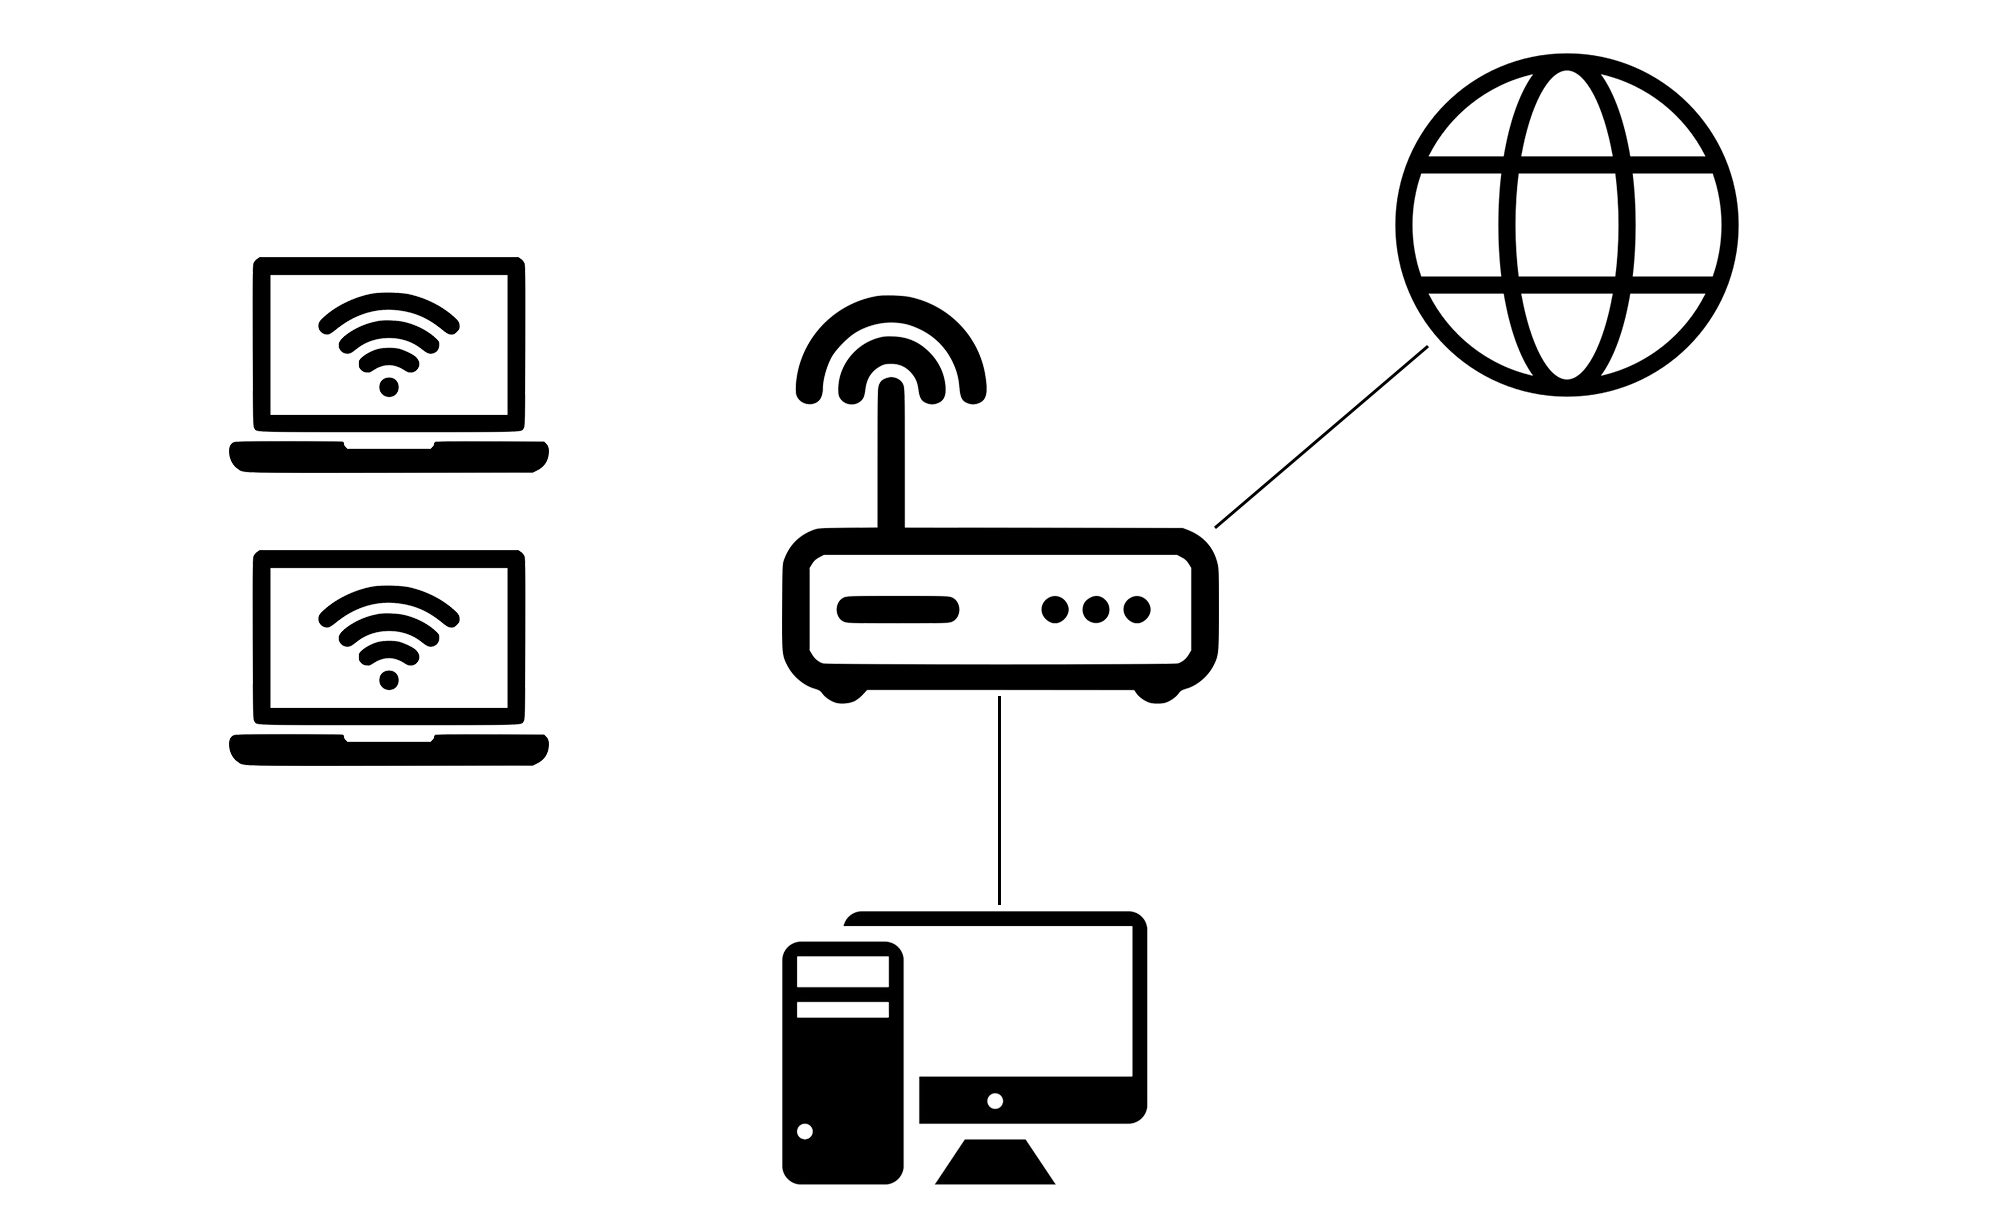
\includegraphics[width=\linewidth]{topology.png}
    \caption{Figura 1: Uma rede doméstica com 3 dispositivos: Um notebook Lenovo, um macbook air e um desktop}
\end{figure}

\subsection{Equipamentos}

\begin{itemize}
    \item Desktop
    \begin{itemize}
        \item Processador: Ryzen 5 3600 @ 3.60 GHz
        \item Memória RAM: 16GB DDR4 3000Mhz
        \item Sistema Operacional: Windows 10
        \item Adaptador Ethernet: Realtek PCIe GBE Family Controller
    \end{itemize}
    \item Macbook
    \begin{itemize}
        \item Processador: Intel i5 3600 @ 3.60 GHz
        \item Memória RAM: 8 GB LPDDR3 1600 MHz
        \item Sistema Operacional: OSX Mojave
        \item Adaptador Wireless: 802.11ac
    \end{itemize}
    \item Notebook Lenovo S30
    \begin{itemize}
        \item Processador: Intel® Core™ i5-1035G1 Quad Core 1.0 GHz com Turbo Max até 3.6 GHz
        \item Memória RAM: 4 GB DDR4 2666 MHz + 16 GB Optane (4 GB soldado + 1 slot livre)
        \item Sistema Operacional: Windows 10
        \item Adaptador Wireless: 802.11ac
    \end{itemize}
    \item Modem
    \begin{itemize}
        \item Modelo: TP-Link WR740N
        \item Frequência: 2.4 GHz
    \end{itemize}
\end{itemize}

\section{Monitoramento}

\subsection{Probe}

\end{document}  